% Options for packages loaded elsewhere
\PassOptionsToPackage{unicode}{hyperref}
\PassOptionsToPackage{hyphens}{url}
%
\documentclass[
]{article}
\usepackage{lmodern}
\usepackage{amssymb,amsmath}
\usepackage{ifxetex,ifluatex}
\ifnum 0\ifxetex 1\fi\ifluatex 1\fi=0 % if pdftex
  \usepackage[T1]{fontenc}
  \usepackage[utf8]{inputenc}
  \usepackage{textcomp} % provide euro and other symbols
\else % if luatex or xetex
  \usepackage{unicode-math}
  \defaultfontfeatures{Scale=MatchLowercase}
  \defaultfontfeatures[\rmfamily]{Ligatures=TeX,Scale=1}
\fi
% Use upquote if available, for straight quotes in verbatim environments
\IfFileExists{upquote.sty}{\usepackage{upquote}}{}
\IfFileExists{microtype.sty}{% use microtype if available
  \usepackage[]{microtype}
  \UseMicrotypeSet[protrusion]{basicmath} % disable protrusion for tt fonts
}{}
\makeatletter
\@ifundefined{KOMAClassName}{% if non-KOMA class
  \IfFileExists{parskip.sty}{%
    \usepackage{parskip}
  }{% else
    \setlength{\parindent}{0pt}
    \setlength{\parskip}{6pt plus 2pt minus 1pt}}
}{% if KOMA class
  \KOMAoptions{parskip=half}}
\makeatother
\usepackage{xcolor}
\IfFileExists{xurl.sty}{\usepackage{xurl}}{} % add URL line breaks if available
\IfFileExists{bookmark.sty}{\usepackage{bookmark}}{\usepackage{hyperref}}
\hypersetup{
  pdftitle={Linear Regression},
  pdfauthor={Jeremy Teitelbaum},
  hidelinks,
  pdfcreator={LaTeX via pandoc}}
\urlstyle{same} % disable monospaced font for URLs
\usepackage{graphicx}
\makeatletter
\def\maxwidth{\ifdim\Gin@nat@width>\linewidth\linewidth\else\Gin@nat@width\fi}
\def\maxheight{\ifdim\Gin@nat@height>\textheight\textheight\else\Gin@nat@height\fi}
\makeatother
% Scale images if necessary, so that they will not overflow the page
% margins by default, and it is still possible to overwrite the defaults
% using explicit options in \includegraphics[width, height, ...]{}
\setkeys{Gin}{width=\maxwidth,height=\maxheight,keepaspectratio}
% Set default figure placement to htbp
\makeatletter
\def\fps@figure{htbp}
\makeatother
\setlength{\emergencystretch}{3em} % prevent overfull lines
\providecommand{\tightlist}{%
  \setlength{\itemsep}{0pt}\setlength{\parskip}{0pt}}
\setcounter{secnumdepth}{-\maxdimen} % remove section numbering
% latex macros

\newcommand{\R}{\mathbf{R}}
\hypersetup{colorlinks=true,linkcolor=blue}

\title{Linear Regression}
\author{Jeremy Teitelbaum}
\date{March 24, 2020}

\begin{document}
\maketitle

\hypertarget{linear-regression}{%
\section{Linear Regression}\label{linear-regression}}

\hypertarget{introduction}{%
\subsection{Introduction}\label{introduction}}

Linear regression is a prototypical machine learning algorithm. To get a
feel for it, let's look at some data on the relationship between engine
size and gas mileage for a group of cars (see
\href{https://archive.ics.uci.edu/ml/datasets/Auto+MPG}{UCI-auto-mpg}
or, for a nicely formatted csv version,
\href{https://www.kaggle.com/uciml/autompg-dataset}{kaggle-auto-mpg}).

In its simplest version, we start with the assumption that a particular
quantity \(y\) that we would like to understand depends on a quantity
\(x\) that we know through a linear relationship: Also, we have
\(x\in\R\).

Here is a picture:

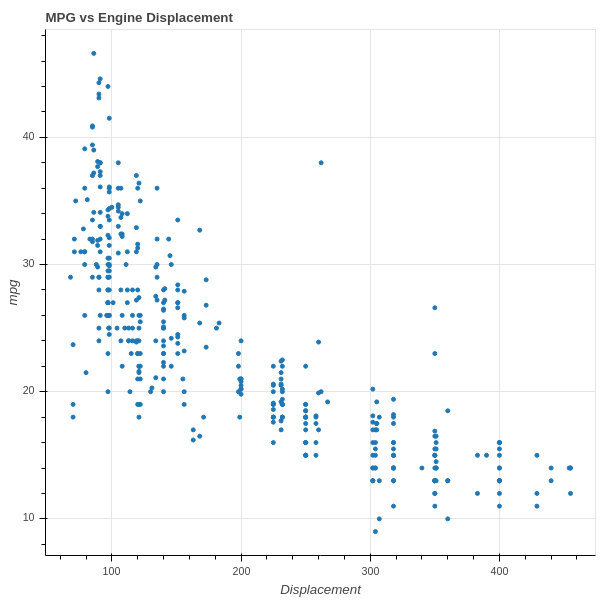
\includegraphics[width=4.16667in,height=\textheight]{../img/mpg-vs-displacement.png}\{class=``center''\}

\end{document}
